%=========================================================================
% Start of activity on piece wise defined functions and max/min
%=========================================================================
\preClass{Title}

\begin{problem}
\item The graph of a function, $g$, is shown shown below:

  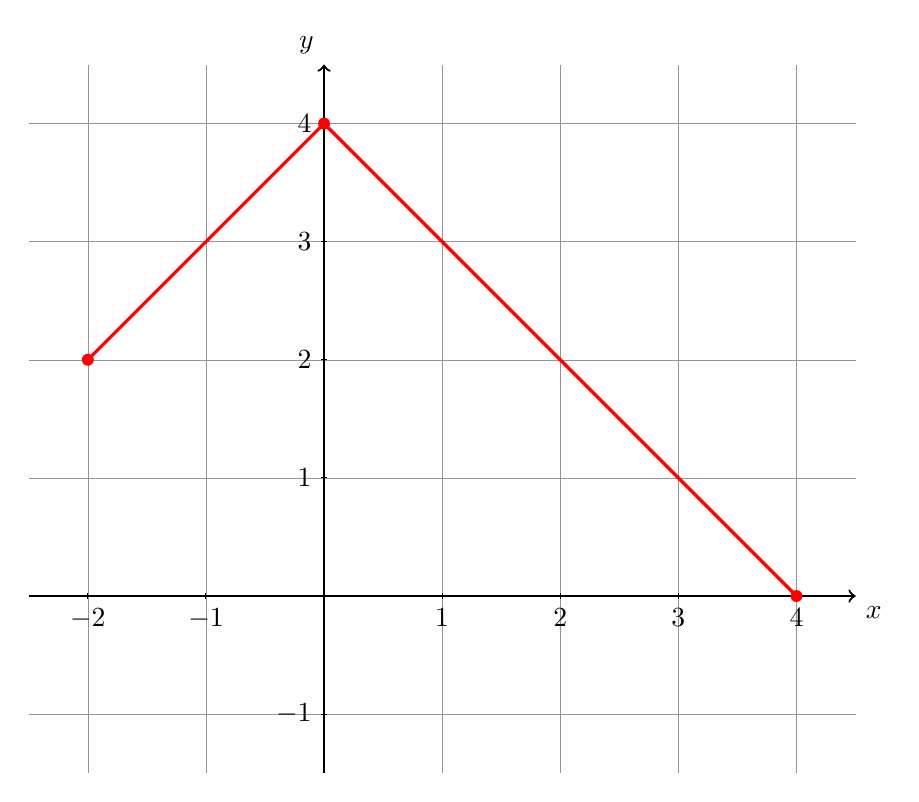
\begin{tikzpicture}[y=1.5cm, x=1.5cm,font=\sffamily]
    % ticks
    \draw[step = 1, gray, very thin,opacity=0.85] (-2.5, -1.5) grid ( 4.5, 4.5);
 	% axis
	\draw[thick,->] (-2.5,0) -- coordinate (x axis mid) (4.5,0) 
          node[anchor = north west] {$x$};
    \draw[thick,->] (0,-1.5) -- coordinate (y axis mid) (0,4.5) 
          node[anchor = south east] {$y$};
    \foreach \y in {-1,1,2,3,4} {
      \draw (1pt, \y) -- (-1pt, \y) node[anchor = east] {$\y$};
    }
    \foreach \x in {-2,-1,1,2,3,4} {
      \draw (\x,1pt) -- (\x,-1pt) node[anchor = north] {$\x$};
    }
    % Draw the function
    \draw [red, very thick] plot coordinates {(-2,2) (0,4) (4,0)};
    \fill[red] (-2, 2) circle [radius=0.5ex];
    \fill[red] ( 0, 4) circle [radius=0.5ex];
    \fill[red] ( 4,0) circle [radius=0.5ex];
  \end{tikzpicture}

  \begin{subproblem}
  \item Determine the domain and range of the function.
    \vfill
  \item Determine the formula for the function if $x\geq -2$ and
    $x<0$.
    \vfill
  \item Determine the formula for the function if $x> 0$ and
    $x\leq 4$.
    \vfill
  \item For what values of $x$ is the function increasing?
    \vspace{2em}
  \item For what values of $x$ is the function decreasing?
    \vspace{2em}
  \end{subproblem}

\end{problem}


\actTitle{title}
\begin{problem}
\item 
  \begin{subproblem}
    \item

  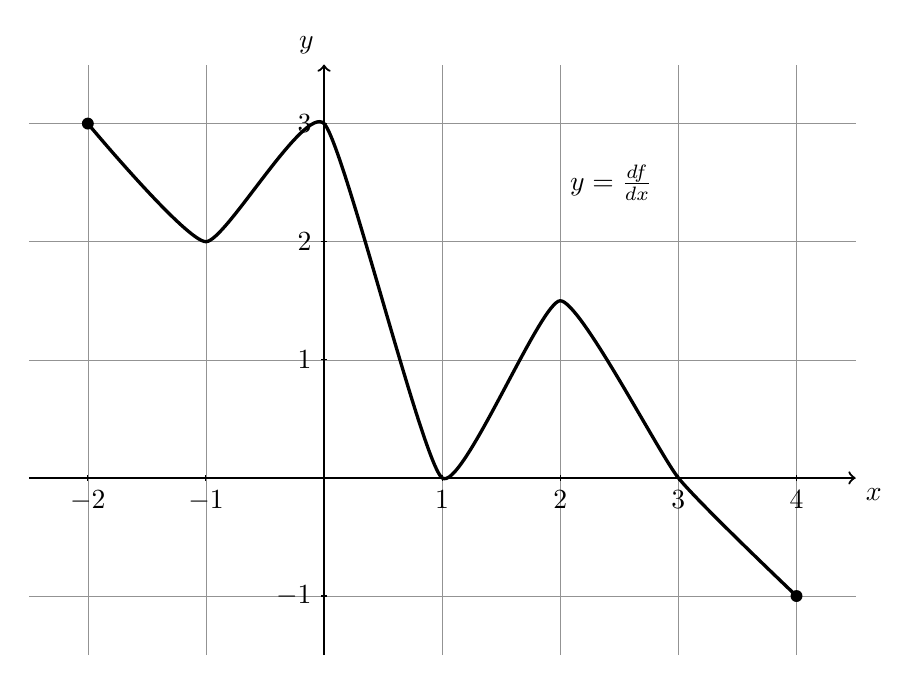
\begin{tikzpicture}[y=1.5cm, x=1.5cm,font=\sffamily]
    % ticks
    \draw[step = 1, gray, very thin,opacity=0.85] (-2.5, -1.5) grid ( 4.5, 3.5);
 	% axis
	\draw[thick,->] (-2.5,0) -- coordinate (x axis mid) (4.5,0) 
          node[anchor = north west] {$x$};
    \draw[thick,->] (0,-1.5) -- coordinate (y axis mid) (0,3.5) 
          node[anchor = south east] {$y$};
    \foreach \y in {-1,1,2,3} {
      \draw (1pt, \y) -- (-1pt, \y) node[anchor = east] {$\y$};
    }
    \foreach \x in {-2,-1,1,2,3,4} {
      \draw (\x,1pt) -- (\x,-1pt) node[anchor = north] {$\x$};
    }
    % Draw the function
    \draw [black, very thick] plot [smooth, tension=0.3] coordinates {
      (-2,3) (-1,2) (0,3) (1,0) (2,1.5) (3,0) (4,-1)};
    \node[anchor = west] at (2.0,2.5) {$y=\frac{df}{dx}$};
    \fill (-2, 3) circle [radius=0.5ex];
    \fill ( 4,-1) circle [radius=0.5ex];
  \end{tikzpicture}

  \end{subproblem}
\end{problem}

\postClass

\begin{problem}
\item Briefly state two ideas from today's class.
  \begin{itemize}
  \item 
  \item 
  \end{itemize}
\item 
  \begin{subproblem}
    \item
  \end{subproblem}
\end{problem}


%%% Local Variables:
%%% mode: latex
%%% TeX-master: "../labManual"
%%% End:

